\documentclass[11pt]{article}
\usepackage{fullpage}
\usepackage{graphicx}
\title{La Cocina de Kojo. Soluci\'on}
\author{Ariel Coto Santiesteban, C-412}
\begin{document}
\maketitle
\section{Orden del problema}
La cocina de Kojo es uno de los puestos de comida r\'apida en un centro
comercial. El centro comercial est\'a abierto entre las 10:00 am y las 9:00 pm cada
d\'ia. En este lugar se sirven dos tipos de productos: s\'andwiches y sushi. Para los
objetivos de este proyecto se asumir\'a que existen solo dos tipos de consumidores:
unos consumen solo s\'andwiches y los otros consumen solo productos de la gama
del sushi. En Kojo hay dos peri\'odos de hora pico durante un d\'ia de trabajo;
uno entre las 11:30 am y la 1:30 pm, y el otro entre las 5:00 pm y las 7:00
pm. El intervalo de tiempo entre el arribo de un consumidor y el de otro no es
homog\'eneo pero, por conveniencia, se asumir\'a que es homog\'eneo. El intervalo
de tiempo de los segmentos homog\'eneos, distribuye de forma exponencial.
Actualmente dos empleados trabajan todo el d\'ia preparando s\'andwiches y
sushi para los consumidores. El tiempo de preparaci\'on depende del producto en
cuesti\'on. Estos distribuyen de forma uniforme, en un rango de 3 a 5 minutos
para la preparaci\'on de s\'andwiches y entre 5 y 8 minutos para la preparaci\'on de
sushi.
El administrador de Kojo est\'a muy feliz con el negocio, pero ha estado recibiendo 
quejas de los consumidores por la demora de sus peticiones. \'El est\'a 
interesado en explorar algunas opciones de distribuci\'on del personal para reducir
el n\'umero de quejas. Su inter\'es est\'a centrado en comparar la situaci\'on actual con
una opci\'on alternativa donde se emplea un tercer empleado durante los peri\'odos
m\'as ocupados. La medida del desempe\~no de estas opciones estar\'a dada por el
porciento de consumidores que espera m\'as de 5 minutos por un servicio durante
el curso de un d\'ia de trabajo.
Se desea obtener el porciento de consumidores que esperan m\'as de 5 minutos
cuando solo dos empleados est\'an trabajando y este mismo dato agregando un
empleado en las horas pico.
\section{Soluci\'on}
\subsection{Principales variables}
El problema se\~nala tres variables aleatorias a generar fundamentales:
\begin{enumerate}
	\item[-] $t_{arribo}$ : el tiempo del pr\'oximo arribo al sistema 
	\item[-] $s$ : la selecci\'on entre s\'andwich o sushi en el men\'u
	\item[-] $t_{p}$ : el tiempo de preparaci\'on del plato.
\end{enumerate} 
Teniendo en cuenta que solamente existen dos tipos de platos podemos tambien usar una Bernoulli en vez de una uniforme de 0 a 1. Como existen horarios picos, la soluci\'on que se presenta recibe como par\'ametro los lambdas para ambos horarios. Como el cliente desea testear adem\'as si emplear otro trabajador en los horarios picos, en la entrada del modelo se encuentra un booleano q representa si emplear un trabajador extra o no.
El tiempo se tom\'o en segundos.
El sistema cuenta con dos colas:
\begin{enumerate}
	\item[-] $S_{entry}$ : representa la cola de clientes a antender en la que se guarda el tiempo de llegada de cada cliente, y 
	\item[-] $S_{out}$ : almacena los tiempos que tuvo que esperar cada cliente para que lo antendieran.
\end{enumerate}
La respuesta al problema es el por ciento de los clientes de $S_{out}$ que esperaron m\'as 5 minutos.
Adem\'as, se cuenta con un array $worker\_busy$ booleano, que muestra si un trabajador est\'a ocupado o no.
\subsection{Principales ideas}
B\'asicamente el algoritmo es el siguiente:
\begin{enumerate}
	\item Se abre la tienda
	\item Si hay alguien en la cola, pasa a ser atendido por el primer trabajador libre.
	\item Si ya termin\'o el trabajador i, se pasa al paso $2$.
	\item Si es hora pico se agrega si se desea medir con un trabajador m\'as, si no, se elimina al tercer
	trabajador si existe.
	\item Si es hora de cerrar se terminan de atender a los clientes de la cola y no se admiten m\'as arribos.
\end{enumerate}
Los dos eventos esenciales en este problema son:
\begin{enumerate}
	\item[-] Llegada de un cliente al restaurante
	\item[-] Salida de un cliente del restaurante
\end{enumerate}
Por tanto, el sistema se basa en ejecutar el primero que ocurra en el tiempo, teniendo en cuenta las condiciones 
del momento, como por ejemplo, si $t_{arribo} < t_{s}$(tiempo de salida), pero $t_{arribo} > T$ (tiempo de cierre), entonces no hay m\'as arribos, y se pasa a la salida del cliente.
\section{El Modelo}
%Se model\'o en horarios no picos con 2 servidores en paralelo, y en los picos con 3.
\textbf{\Large Estados:}
\begin{enumerate}
	\item [-] Llegada de un cliente al restaurante.
	\item [-] Entrega al cliente de su pedido por el trabajador i-\'esimo (salida del sistema).
\end{enumerate}
\textbf{\Large Variables:}
\begin{enumerate}
	\item [-] $t$ (tiempo de la simulaci\'on)
	\item [-] $t_{arribo}$ (tiempo del pr\'oximo arribo de un cliente al restaurante)
	\item [-] $t_{out}(i)$ (tiempo de salida del cliente del trabajador i-\'esimo)
	\item [-] $W(i)$ (estado del trabajador i-\'esimo,ocupado o libre)
	\item [-] $opened$ (boolean, estado de la tienda, abierta o cerrada)
	\item [-] $S_{entry}$ (cola de clientes a atender en la que se guarda el tiempo de llegada de cada cliente)
	\item [-] $S_{out}$ (cola, tiempo que estuvo cada cliente en la cola)
	\item [-] $C(i)$ (cantidad de clientes atendidos por el trabajador i)
	\item [-] $N_a$ (n\'umero de arribos al sistema)
	\item [-] $p$ (proporci\'on para escoger entre sushi y s\'andwich)
	\\
\end{enumerate}
\textbf{\Large Modelo:}\\\\
Se utilizar\'a la notaci\'on $I_0$ para significar $1\leq i \leq 2$ e $I_1$ para $1\leq i \leq 3$.
Se utilizar\'a la funci\'on $is\_rush\_hour(t)$ para determinar si el tiempo $t$ est\'a en el intervalo de hora pico.
\begin{itemize}
	\item Inicializaci\'on 
	\begin{enumerate}
		\item $opended = True$
		\item $t = N_a = 0$
		\item $W(i)  = False$ para $I_0$
		\item $S_{entry} = S_{out} = (0)$ 	
		\item  Generar $T_i$ y hacer $t_{arribo} = T_i$
		\item  $t_{out}(i)= \infty$ para $I_1$
	\end{enumerate}
	\item Caso: Llega un cliente al restaurante (si $t_{arribo} = $ min($t_{arribo},t_{out}(i)$ para $I_{1}$) y $t_{arribo} < T$)
		\begin{enumerate}
		\item $t = t_{arribo}$
		\item $N_a = N_a + 1$
		\item $S_{entry} $ a\~nadir $t$ moment\'aneamente
		\item Si $\exists i$ $ W(i)=False$, sea $i$ el m\'inimo
		\begin{enumerate}
			\item [-]$W(i) = True$
			\item [-]$C(i) = C(i) + 1$
			\item [-] $k = S_{entry}[0] $ se extrae su primer elemento
			\item [-]$S_{out}$ a\~nadir $t - k$
			\item [-]Generar $P$ que distribuye como $U(0,1)$. Si $P>p$ hacer $sushi = True$, si no $sushi= False$
			\item [-]Si $sushi = True$, generar $S_u$ que distribuye $U(5,8)$ y hacer $t_{out}(i)=t+S_u$, si no generar $S_a$ que distribuye $U(3,5)$ y hacer $t_{out}(i)=t+S_a$
		\end{enumerate}
	\item Si $is\_rush\_hour(t) = True$, generar $T_{rush}$ y hacer $t_{arribo} = t + T_{rush}$,
		\begin{enumerate}
			\item [-] Si queremos probar con un 3er trabajador y no se ha agregado, se agrega.
		\end{enumerate}
	\item Si no, generar $T_{no\_rush}$ $t_{arribo} = t + T_{no\_rush}$
		\begin{enumerate}
			\item [-] Si hay trabajando 3 personas y el 3ro ya termi\'o, entonces se remueve
		\end{enumerate}
	\end{enumerate}
	\item Caso: Se libera el tarbajador j (si $t_{j} = $ min($t_{arribo},t_{out}(i)$ para $I_{1}$) \'o ($\exists i$ $ W(i)=True$ and $opened=False$))
	\begin{enumerate}
		\item  $t=t_j$
		\item  Si $S_{entry} = (0)$
		\begin{enumerate}
			\item [-] $W(j)=False$ y $t_{out}(j) = \infty$
		\end{enumerate}
		\item Si no
		\begin{enumerate}
			\item [-]$k = S_{entry}[0] $ se extrae su primer elemento
			\item [-]$S_{out}$ a\~nadir $t - k$
			\item [-]Generar $P$ que distribuye como $U(0,1)$. Si $P>p$ hacer $sushi = True$, si no $sushi= False$
			\item [-]Si $sushi = True$, generar $S_u$ que distribuye $U(5,8)$ y hacer $t_{out}(i)=t+S_u$, si no generar $S_a$ que distribuye $U(3,5)$ y hacer $t_{out}(i)=t+S_a$
		\end{enumerate}
	\end{enumerate}
	\item Caso: Cierre de la tienda ($t\geq T$ \'o $t_{arribo}\geq T$)
		\begin{enumerate}
			\item [-] $opened = False$
		\end{enumerate}
	
\end{itemize}
\section{Implementaci\'on}
Para correr el sistema se debe ejecutar en la carpeta del proyecto \emph{python3 main.py}y seguir con las instrucciones que le aparecen. el main.py ejecutar\'a 100 simulaciones del problema y guarda\'a los resultados en el archivo \emph{Kojo\_simulations.db}. Para mostrar los resultados deberá ejecutar \emph{python3 kojo\_plotter.py}.
\section{Consideraciones}
Los resultados de las experimentaciones se almacenaron en Kojo\_simulations.db, la cual es una base de datos de sqlite. En este .db existen 2 tablas, \emph{three\_workers\_waits} y \emph{two\_workers\_waits}, las cuales almacenan los resultados de experimentar con 2 trabajadores y con tres en las horas picos. Los datos q se almacenan son: \emph{waits} (tiempo de espera de un cliente), \emph{cnt\_simulations} (cantidad de simulaciones realizadas en el experimento), \emph{rush\_EX} (la media utilizada para simular las horas pico), la otra media \emph{normal\_EX}, y \emph{sushi\_prop} que representa la raz\'on de la seleci\'on entre sushi y s\'andwich. 
En general, el comportamiento de los resultados depende mucho de los par\'ametros del sistema. Si la gente pide mucho sushi, m\'as demora va a haber en la cola, al igual que mientras m\'as distantes est\'en las medias de las llegadas de los clientes se va a notar m\'as la diferencia.
\begin{figure}	
	\begin{center}
		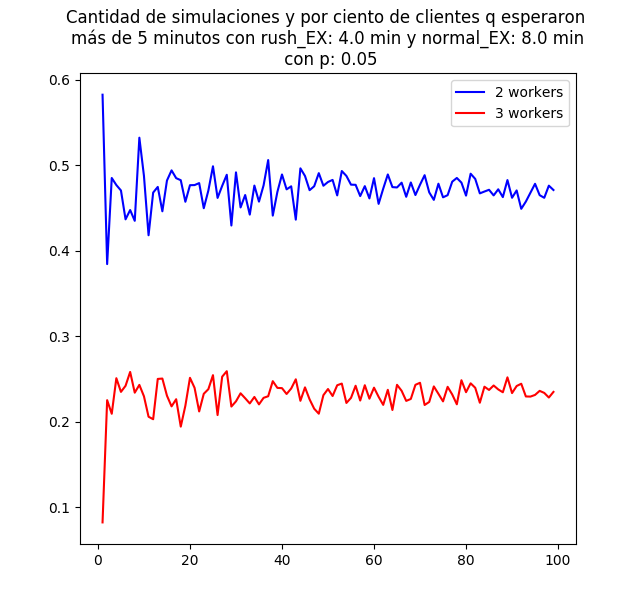
\includegraphics[width=0.5\textwidth]{index}
		\caption{Resultados desde 1 hasta 100 simulaciones}
	\end{center}
\end{figure}

\end{document}